\chapter{Design}

My design for the tool was driven by a determination to combine the best elements of the other visual programming environments and the other works that inspired this project. My tool takes the rich graphical representation of code structure from the Lamdu project but structures it in such a way that each toy language can its own visual structure according to its own rules.

\section{Program visualisation}

The user interface for this tool focuses on what matters - the program that the user has written. Unlike the traditional tools with their split between the text program code and the visualisations, the program code is displayed once in a rich visual manner. When the traditional text-based model is geared around a monospaced grid of characters into which the program code is rigidly put, this application displays program code according to its actual structure and meaning. Individual elements such as method names or number literals are represented textually as normal, but elements are freed from the grid model to display themselves in whatever manner would best explain their meaning to the programmer. The layout and styling of these elements is not fixed but can be changed dynamically due to user input, the correctness of the code within or any other relevant factor that may assist the programmer.

\subsection{Traditional programming model}

In the traditional text-based model, the first stages of both a compiler or an interpreter are lexing and parsing.

\paragraph{Lexing}

The lexer turns the series of characters in the source file into a series of individual tokens, such as an identifier or a number literal, representing individual elements of the code in order. The Lexer will include the line number and character range from the source file of each token so that later compilation steps may give useful error messages that allow the programmer to locate any errors or warnings. Lexing will only fail if the input includes characters or combinations thereof which do not map to any valid token. Languages which do not attach meaning to whitespace characters have lexers which automatically skip over any incoming whitespace without producing any tokens. The only relevance of whitespace in these languages is to signify the end of the previous token and the start of the next one. Lexers in languages which do give meaning to whitespace, such as Python or Haskell, normally produce tokens which abstract over the meaning given (such as to indent and dedent a code block) rather than producing a token for each encountered whitespace character, as there may be multiple whitespace forms which have the same meaning.

\paragraph{Parsing}

The parser then takes the lexed list of tokens and assembles them into a tree structure according to the grammar rules of that language. Parsing fails if the list of tokens does not match this grammar. Languages are defined by their concrete syntax, which includes symbols such as brackets which are used by the programmer to indicate their intent. The parsed form of the program no longer needs to include these symbols and is called the Abstract Syntax Tree. This tree is formed of individual nodes representing each different element of the language, such as an array access, a method call, a function block or an value literal. Those symbols necessary to clarify programmer intent (such as the brackets commonly used to represent a function call) are no longer required explicitly in the AST.

\begin{figure}[H]
\centering
\begin{verbatim}
method myFunction (x, y) {
    let z := x + y / 4
    return z
}
\end{verbatim}
\caption{Traditional text code sample}
\label{fig:tradcode} % insert suitable label, this is used to refer to a fig from within the text as shown above
\end{figure}

\begin{figure}[H]
\centering
\begin{verbatim}
program ::= method*

method ::= "method" ident "(" method_args ")" "{" statement* "}"

method_args ::= ε | ident ( "," ident )*

statement ::= let_statement | return_statement

let_statement ::= "let" ident ":=" expression

return_statement ::= "return" expression

expression ::= primary_expression | binary_expression

primary_expression ::= value_expression | literal_expression

value_expression ::= ident

literal_expression ::= number

binary_expression ::= expression op expression

op ::= "+" | "-" | "/" | "*"

ident ::= [a-zA-Z]+

number ::= [0-9]+
\end{verbatim}
\caption{Language grammar of code in Figure \ref{fig:tradcode} in Extended Backus-Naur Form}
\label{fig:tradgrammar} % insert suitable label, this is used to refer to a fig from within the text as shown above
\end{figure}

\begin{figure}[H]
\centering
\begin{verbatim}
METHOD, IDENT(myFunction), LPAREN, IDENT(x), COMMA, IDENT(y), RPAREN,
LBRACE, LET, IDENT(z), ASSIGN, IDENT(x), OP_ADD, IDENT(y) OP_DIV,
NUMBER, RETURN, IDENT(z), RBRACE
\end{verbatim}
\caption{Lexer output of code in Figure \ref{fig:tradcode} according to grammar in Figure \ref{fig:tradgrammar}}
\label{fig:tradlexed} % insert suitable label, this is used to refer to a fig from within the text as shown above
\end{figure}

\begin{figure}[H]
\centering
\begin{verbatim}
(method
    (ident "myFunction")
    (cons
        (ident "x")
        (ident ("y")
    )
    (cons
        (let_statement
            (ident "z")
            (binary_expression
                "+"
                (value_expression "x")
                (binary_expression
                    "/"
                    (value_expression "y")
                    (number "4") 
                )
            )
        )
        (return_statement (value_expression "z"))
    )
\end{verbatim}
\caption{Parser output from lexed tokens in Figure \ref{fig:tradlexed} according to grammar in Figure \ref{fig:tradgrammar} (in lisp notation)}
\label{fig:tradparsed} % insert suitable label, this is used to refer to a fig from within the text as shown above
\end{figure}

\subsection{Abstract Syntax Tree visualisation}

It is this Abstract Syntax Tree that that forms the basis of the visual representation of programs in this tool. The AST the final and unambiguous representation of how the computer understands the user’s program. By displaying it directly, the gap between how the programmer and the computer can understand a program is removed. All that is left is the essential complexity of what the program actually does.

\begin{figure}[H]
\centering
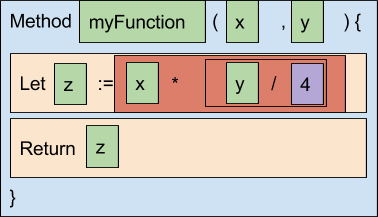
\includegraphics[scale=0.5]{graphics/astdesign} % e.g. insert ./image for image.png in the working directory, adjust scale as necessary
\caption{Visual representation of a Method AST node}
\label{fig:astdesign} % insert suitable label, this is used to refer to a fig from within the text as shown above
\end{figure}

\begin{table}[H]
\centering
\caption{AST node block colour key}
\label{fig:astcolourkey}
\begin{tabular}{|l|l|}
\hline
\textit{\textbf{Colour}} & \textit{\textbf{Node}} \\ \hline
Green                    & Ident                  \\ \hline
Purple                   & Literal                \\ \hline
Cream                    & Statement              \\ \hline
Red                      & Binary Expression      \\ \hline
Blue                     & Method                 \\ \hline
\end{tabular}
\end{table}

At one extreme, AST visualisations could be in the same format as the original text-based source code. This AST-to-source conversion step is used in source code formatting tools, which apply a single canonical representation of how the code should be formatted without changing its structure or meaning. At the other there are representations which are entirely visual and could not be easily written into text. This is the concept of the Scratch programming language, as there is never a textual form to a program. When Scratch programs are saved to disk, they are converted into a JSON format which preserves the structure of the AST along with the positioning of script elements on the script canvas.

As this tool is intended to act as a stepping stone to ‘real’ programming, an intermediate form is used where the code is displayed in manner which is recognisable from text-based programming. However, each element of the program is in its own display block which can grow and shrink according to need. These blocks are nested in accordance with the program structure and each code block has its own unique visual representation which is drawn whenever encountered in the AST. Elements of the concrete syntax, such as keywords and symbols, are drawn in these visual representations so that the meaning and behaviour of the code is clear to the user. Unlike the traditional model, there is only one unambiguous representation of the AST as there can be no minor changes to whitespace.

\subsection{AST editing}

\begin{figure}[H]
\centering
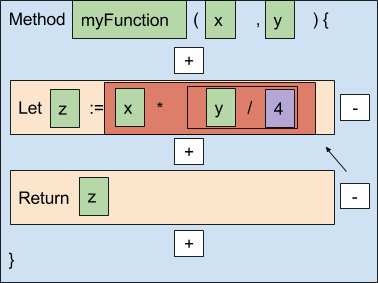
\includegraphics[scale=0.5]{graphics/aststatement1} % e.g. insert ./image for image.png in the working directory, adjust scale as necessary
\caption{Visual representation of Statement list editing in the AST}
\label{fig:aststatment1} % insert suitable label, this is used to refer to a fig from within the text as shown above
\end{figure}

\begin{figure}[H]
\centering
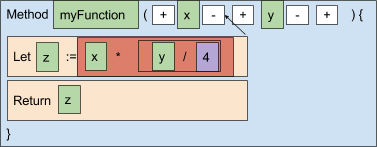
\includegraphics[scale=0.5]{graphics/astarg1} % e.g. insert ./image for image.png in the working directory, adjust scale as necessary
\caption{Visual representation of Method argument list editing in the AST}
\label{fig:astarg1} % insert suitable label, this is used to refer to a fig from within the text as shown above
\end{figure}

Moving the cursor over a code block reveals additional visual elements which could not be replicated in the text-based model. A method includes a list of statements, and upon being moused over it will show buttons to insert new statements at all points in the list along with buttons to delete the statements which already exist. These buttons will appear gradually, with the visual blocks changing position and size smoothly to accommodate them. Buttons appearing out of nowhere and moving the code blocks instantaneously would be visually jarring, difficult to use and hard for a novice to follow. The buttons must be visually distinct from code blocks so that the user understands that they are not parts of the program. Their simple symbols and positioning describe their purpose with minimal intrusion. It is key for the usability of the system that these visual elements are common across and within each of the toy language specifications. While the languages themselves may have different semantics and structure, the way that the user interacts with them should be the same. Once the user is confident playing with one toy language, they should be able to tackle any other one. In addition, having common editing interfaces minimises the effort required to create a toy language, while ensuring that the single implementation is as optimal as possible.

\paragraph{Insertion of new elements}

Adding new program content involves a combination of text input and visual selection. Where Scratch requires the user to drag and drop program elements from a toolbox at the side of the script page, this tool allows keyboard input to select the element to be added. Using the concrete syntax of the language, the user's text input can narrow down and then select an element type from a list of all of the possible types that would match the grammar. For example, when a new statement is added, only statement types are shown. It simply is not possible for a user to insert an invalid node. The user interface displays the name of the grammatical construct, thereby indirectly teaching the user about the meaning of different element types. For instance, in a sequential language they will see and learn what an expression is versus a statement, or how in a purely functional language everything is an expression.

\begin{figure}[H]
\centering
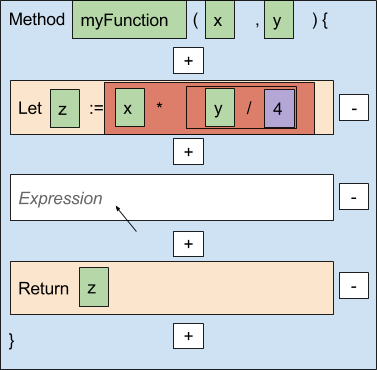
\includegraphics[scale=0.5]{graphics/astentry1} % e.g. insert ./image for image.png in the working directory, adjust scale as necessary
\caption{Visual representation of an empty AST node location}
\label{fig:astentry1} % insert suitable label, this is used to refer to a fig from within the text as shown above
\end{figure}

\begin{figure}[H]
\centering
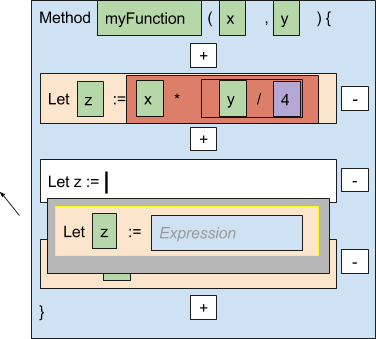
\includegraphics[scale=0.5]{graphics/astentry2} % e.g. insert ./image for image.png in the working directory, adjust scale as necessary
\caption{Visual representation of inserting a new Let statement node}

From the text already entered, the Let statement is the only valid and displayed option.
\label{fig:astentry2} % insert suitable label, this is used to refer to a fig from within the text as shown above
\end{figure}

\section{Program change tracking}

Standard and programming text editors include change tracking functionality in the form of the undo and redo operations. Each change to the program can be represented simply as a series of inserted and deleted characters at certain locations in the file. This functionality is trivial to implement and is not at all specific to computer programming, as it is just as useful when creating a traditional human-language text document.

Implementing undo and redo operations in a visual editor requires a finer degree of change management. Before and after each change, the program code and AST will be in a valid state. Each possible change can be represented in as a discrete, complete change to the tree structure of the program: an attribute modification (such as renaming an identifier), a node replacement or an insertion or deletion from a list of nodes. This change tracking system is core to the application and can represent changes to any valid toy language specification. Re-implementing this change management system for each toy language would be wasteful, so the change management system is agnostic to the actual grammatical structure. Each toy language defines a series of language elements which can have other elements as attributes or in a variety of lists. The change tracking system simply records the elements involved in the change, along with details such as the name of the attribute or the name and index of the list change. 

For maximum flexibility, each user operation on the AST is first calculated as a change and only then is it applied. Calculating the change first means that there will only be one single change implementation system, regardless of the source of the change. Each change can be reversed to create an equivalent but opposite change that will undo that action. As the user modifies their program, a list of the changes they have made is created. When the user requests an undo operation, the most recent change can be retrieved, reversed and then applied to the program. The original change that was undone is added to a list of undone changes. The redo operation takes the most recently undone change and applies it once again to the program. 

This change management mechanism is key for the collaborative working tertiary objective. Text-based program collaboration is done through version control systems such as Git which are only applied when the user requests it, as there is no guarantee that the program is in a valid state at any time. This static model of collaboration stands in contrast to the approach now available in online document editing systems, where it is possible to watch other users edit the same document in real time. This is possible as human documents are unstructured data and there is no 'valid' form for a computer to depend upon. Editing clashes may occur but the computer will simply leave it up the humans to make sense of it and correct it.

\section{Program execution}

Being able to visualise and edit programs is useful but it is not enough to complete it as a programming education tool. For that, it must be necessary for the programs to be executed within the application, thereby allowing execution to be taught and visualised alongside the program structure.

\subsection{Interpreter option}

There were three basic choices available for executing the program code. The first is to interpret it directly, as with scripting languages such as JavaScript and Python. An interpreter works on the AST of a program, produced by the lexing and parsing stages in text-based programming. Each program component type provides an evaluation method which calls its children recursively until leaf nodes are encountered. When all of the operands are available for an execution, such as an operator application or a function call, this is performed and the node is replaced by its return value.

Recursively the entire tree is evaluated, while the interpreter provides an environment so that variables can be assigned and then accessed and evaluated later. While the entire program will be lexed and parsed before execution, each line of code will only be executed one after another. Functions and other values and elements can only be referenced after the interpreter has reached them and added them to the environment using that element's evaluation function.

\begin{figure}[H]
\centering
\begin{verbatim}
my_string = "hello world"
string_length = len(my_string)
print(string_length + 4)
\end{verbatim}
\caption{Example of Python 3 code}
\label{fig:pythoncode} % insert suitable label, this is used to refer to a fig from within the text as shown above
\end{figure}

\begin{figure}[H]
\centering
\begin{verbatim}
Original source code: my_string = "hello world"

Evaluation step 0
Input: (assignment "my_string" (string_literal "hello world"))
Interpreter environment:
{ variables: {}, globals: print(), len(), … }
Evaluation step 1
Input: ()
Interpreter environment:
{ variables: {"my_string": "hello world"}, globals: print(), len(), … }
\end{verbatim}
\caption{Evaluation of first line of code in Figure \ref{fig:pythoncode}}
\label{fig:pythoneval1} % insert suitable label, this is used to refer to a fig from within the text as shown above
\end{figure}

\begin{figure}[H]
\centering
\begin{verbatim}
Original source code: string_length = len(my_string)

Evaluation step 0
Input: (assignment
            "string_length"
            (function_call "len" (value_expression "my_string"))
        )
Interpreter environment:
{ variables: {"my_string": "hello world"}, globals: print(), len(), … }

Evaluation step 1
Input: (assignment
            "string_length"
            (function_call "len" (eval_result "hello world"))
        )
Interpeter environment:
{ variables: {"my_string": "hello world"}, globals: print(), len(), … }

Evaluation step 2
Input: (assignment
            "string_length"
            (eval_result "11")
        )
Interpeter environment:
{ variables: {"my_string": "hello world"}, globals: print(), len(), … }

Evaluation step 3
Input: ()
Interpreter environment:
{ variables: {"my_string": "hello world", "string_length": 11},
  globals: print(), len(), … }
\end{verbatim}
\caption{Evaluation of second line of code in Figure \ref{fig:pythoncode}}
\label{fig:pythoneval2} % insert suitable label, this is used to refer to a fig from within the text as shown above
\end{figure}

\begin{figure}[H]
\centering
\begin{verbatim}
Original source code: print(string_length + 4)

Evaluation step 0
Input: (function_call
            "print"
            (binary_expression "+" (value_expression "string_length") "4")
        )
Interpreter environment:
{ variables: {"my_string": "hello world", "string_length": 11},
  globals: print(), len(), … }

Evaluation step 1
Input: (function_call
            "print"
            (binary_expression "+" (eval_result "11") "4")
        )
Interpreter environment:
{ variables: {"my_string": "hello world", "string_length": 11},
  globals: print(), len(), … }

Evaluation step 2
Input: (function_call
            "print"
            (eval_result "15")
        )
Interpreter environment
{ variables: {"my_string": "hello world", "string_length": 11},
  globals: print(), len(), … }

()
Interpreter environment
{ variables: {"my_string": "hello world", "string_length": 11},
  globals: print(), len(), … }
Side effects: output "15"
\end{verbatim}
\caption{Evaluation of third line of code in Figure \ref{fig:pythoncode}}
\label{fig:pythoneval3} % insert suitable label, this is used to refer to a fig from within the text as shown above
\end{figure}

Interpretation is a suitable model for scripting languages and it would be eminently feasible to implement a full-scale interpreter for the toy languages within this tool. Each language definition would only need to provide the evaluation methods for each of the AST node types, utilising a common environment system.

However, this approach does not lend itself to the requirement for execution to be rewound and run in reverse. The state of the executing machine is the state of the entire interpreter and as nodes are evaluated they are replaced with their evaluated form. Reversing execution would require keeping track of every single evaluation and storing the replaced value. More pressingly, it would be difficult to implement reversals over control flow, such as loop iterations or conditionals. Being able to reverse execution is only truly useful if it allows programmers to return back to before any incorrect control flow decisions, thereby allowing them to modify their code and have execution continue as planned.

\subsection{Trans-compilation option}

Another available option would be to cross-compile the program code into some other language and then run it in its standard interpreted or compiled form. Code generation from the AST is eminently feasible and so long as readability is not a concern, there should be no problems writing a generator targeting any Turing-complete host language. As this project is intended to run within the web framework, JavaScript would be the natural choice for a target language. It supports a very wide range of programming styles including object-oriented, prototypical, procedural and functional, so writing code generation methods for any toy language should be straightforward. There is also good library support for the JavaScript AST itself \cite{estree}, so it would be possible to transform the toy language AST directly into its JavaScript equivalent rather than requiring the code to be written out to valid source code and then lexed and parsed back into an executable form. Modern browsers are extremely efficient at executing JavaScript code given its importance for modern websites and web applications.

However, as with the interpretation option, support for pausing and rewinding execution of user programs would be limited, if not nonexistent. Given the trivially small size of the expected programs the efficiency of JavaScript execution would be irrelevant. If a user did create a program requiring real computational power it is most likely that they would be ready to move to a real programming language and environment. This use-case can be supported by other features of the application, such as exporting source code for use outside of the learning environment.

\subsection{Virtual machine option}

\subsubsection{Concept}

Implementing the execution pause and rewind functionality is most easily done if there is full control over the state and progress of the executing machine. A virtual machine is a computer program which is designed to interpret instructions in a manner similar to real hardware. Code generation for a language can target a virtual machine architecture in the same way as it can target any real life architecture such as x86 or ARM. How the virtual machine executes these instructions is left to the programmer. These instructions will be lower-level than interpretation steps, acting upon more simple definition of a machine state. This simplicity makes it feasible to track the state of the machine as it executes each instruction. If each change is recorded and is able to be reversed, it will be possible to reverse each execution step perfectly. The deterministic nature of software means that reversing the lowest level of the machine will reverse all higher-level behaviour at the language level, which is exactly what is required for this educational environment.

The essence of the virtual machine is that there will be a series of instructions and a machine state. Each instruction will modify the machine state in a limited and predictable manner. The exact level of abstraction provided by the virtual machine is entirely variable. It would be entirely possible to virtualise a real processor architecture such as x86, ARM or MIPS. At this level, instructions and data are in raw bit and byte form as they are designed to be understood directly by the silicon of the chip. Software simulations are possible and require full byte accuracy of input and output, even if the processing itself is performed at a high level.

The low level nature of these architectures means that while each individual supported instruction may be simple, a great number of them must be implemented entirely correctly for the machine to be able to execute any meaningful programs. There will be multiple copies of some basic instructions to handle the byte-level differences between different value types, such as floating point and integer numbers. The code generation steps for the program would have to produce the same sort of machine code as 'real' and extremely sophisticated compiler systems such as GCC. Implementing these systems from scratch would be a challenging task and would detract from the purpose of this project. It may be slightly easier to implement this if the programming environment were a native application on a traditional full-featured operating system such as Linux, as these tools would be available on the operating system. However, these would not be available on closed 'appliance' platforms such as smart devices and would be wholly inappropriate on the web platform. Similar issues exist for slightly higher-level virtual machine specifications such as the JVM, which avoid some of the device-specific complexity of a real machine architecture but would be needlessly difficult to implement within the web architecture.

\subsubsection{Implementation}

The solution is to create a new specification for a virtual machine perfectly tuned for the requirements of this project. This virtual machine will provide the level of control required for the reversal of execution while leveraging the capabilities of the implementation programming language to perform most computation. Program code is compiled into a series of instructions which are loaded into the machine. At a high level the instruction at the instruction pointer index is fetched and executed, changing the state of the machine and then the cycle repeats, just as a physical processor does. However, individual processing instructions are implemented just as simple functions which take so many arguments and provide a return value. To simplify the specification further the machine is a variation on a stack machine. This means that there is no requirement for instructions simply to manage the limited number of registers that are available in any real-life register machine. Operations are done on the stack - when a function or operation is called the arguments are popped off the stack and then the return value is pushed back on. This approach lends itself to very simple recursive descent code generation of expressions, so for that and other reasons is implemented by other virtual machines such as the JVM.

The mechanism by which the virtual machine executes instructions is the key to fulfilling the requirements for this project. Each machine instruction type is defined in terms of the changes that it makes to a machine state. By this, it means more than just that the instruction to add two values will pop two values off the stack and push the result on. The change is defined based upon the actual current state of the machine at that given point in time. When the instruction is fetched, it is given the entire state of the machine and from this it produces a machine change description. This change description includes the change to the instruction pointer and the actual values pushed off and popped on of the stack amongst others. Once the change information has been produced, it is added to a history list before being applied to the machine state to complete execution. It is therefore similar in concept to the change management system for the program AST, including the ability to reverse a change to perfectly reset the machine state to its previous form. 

\subsection{Virtual machine formal specification}

\subsubsection{Machine}

The machine state $M$ is a tuple $\langle I, P, T, G, C, L \rangle$ where
\begin{itemize}
\item $I$ is the list of machine instructions
\item $P$ is the current instruction pointer value
\item $T$ is a list of stack frames $F_0..F_n$
\item $G$ is the global environment key-value mapping function $k \mapsto s$
\item $C$ is the console state $c_0...c_n$, i.e. a list of individual characters that have been printed
\item $L$ is the global labelling function $l \mapsto P$
\end{itemize}

A stack frame $F$ is a tuple $\langle S, E, R, A \rangle$ where
\begin{itemize}
\item $S$ is the list of stack elements $s_0...s_n$
\item $E$ is the stack environment key-value mapping function $k \mapsto s$
\item $R$ is the return address value, taken from the current instruction pointer during a method call
\item $A$ is the arguments list
\end{itemize}

\subsubsection{Instruction set}

The machine state change caused by each instruction is as follows

\subsubsection{PushStackFrame}

\begin{multline*}
\langle \text{PushStackFrame}; I, p, F_0...F_n, G, C, L\rangle  \\ \mapsto \langle I, p+1, F_0...F_n, \langle \emptyset, [], null, \emptyset\rangle , G, C, L\rangle 
\end{multline*}

\subsubsection{PopStackFrame}
\begin{multline*}
\langle \text{PopStackFrame}; I, p, F_0...F_n, G, C, L\rangle \mapsto \langle I, p+1, F_0...F_{n-1}, G, C, L\rangle 
\end{multline*}
\subsubsection{Push}

\begin{multline*}
\langle \text{Push}\ s; I, p, F_0...\langle s_0...s_n, E, R, A\rangle , G, C, L\rangle  \\ \mapsto \langle I, p+1, F_0...\langle s_0...s_n.s, E, R, A\rangle 
\end{multline*}

\subsubsection{Pop}
\begin{multline*}
\langle \text{Pop}; I, p, F_0...\langle s_0...s_n, E, R, A\rangle , G, C, L\rangle  \\ \mapsto \langle I, p+1, F_0...\langle s_0...s_{n-1}, E, R,  A\rangle , G, C, L
\end{multline*}
\subsubsection{Dup}
\begin{multline*}
\langle \text{Dup}; I, p, F_0...\langle s_0...s_n, E, R, A\rangle , G, C, L\rangle  \\ \mapsto \langle I, p+1, F_0...\langle s_0...s_n.s_n, E, R, A\rangle , G, C, L\rangle 
\end{multline*}
\subsubsection{CallFunction}
\begin{multline*}
\langle \text{CallFunction}\ \langle f\ a\rangle ; I, p, F_0...\langle s_0...s_n, E, R, A\rangle , G, C, L\rangle  \\ \mapsto \langle I, p+1, F_0...\langle s_0...s_{n-a}.f\langle s_{n-a}...s_n\rangle , E, R, A\rangle , G, C, L\rangle 
\end{multline*}
\subsubsection{MethodCall}
\begin{multline*}
\langle \text{MethodCall}\ m \ a; I, p, F_0...\langle s_0...s_n, E, R\rangle , T, G, C, L[m=b]\rangle  \\ \mapsto \langle I, b, F_0...\langle s_0...s_{n-a}, E, p\rangle .\langle \emptyset, [], null, s_{n-a}...s_n\rangle , G, C, L\rangle 
\end{multline*}
\subsubsection{Return}
\begin{multline*}
\langle \text{Return}\ e; I, p, \emptyset, G, C, L[\text{TERMINATE}=t]\rangle \mapsto \langle I, t, \emptyset, G, C, L\rangle 
\end{multline*}
\begin{multline*}
\langle \text{Return}\ {true}; I, p, F_0...\langle u_0...u_n, E, R, A\rangle .\langle s_0...s_n, E, r\rangle , G, C, L\rangle  \\ \mapsto \langle I, r, F_0...F_{n-2}.\langle u_0..u_n.s_n, E, R, A\rangle , G, C, L\rangle 
\end{multline*}
\begin{multline*}
\langle \text{Return}\ false; I, p, F_0...\langle s_0...s_n, E, R, A\rangle , G, C, L\rangle  \\ \mapsto \langle I, r, F_0...F_{n-1}.\langle G, C, L\rangle 
\end{multline*}
\subsubsection{Goto}
\begin{multline*}
\langle \text{Goto}\ l; I, p, T, G, C, L[l=a]\rangle \mapsto \langle I, a, T, G, C, L\rangle 
\end{multline*}
\subsubsection{IfGoto}
\begin{multline*}
\langle \text{IfGoto}\ l; I, p, F_0...\langle s_0...s_{n-1}.\text{TRUTHY}, E, R, A\rangle , G, C, L[l=a]\rangle  \\ \mapsto \langle I, a, F_0...\langle s_0...s_{n-1}, E, R, A\rangle , G, C, L\rangle 
\end{multline*}
\begin{multline*}
\langle \text{IfGoto}\ l; I, p, F_0...\langle s_0...s_{n-1}.\text{FALSY}, E, R, A\rangle , G, C, L[l=a]\rangle  \\ \mapsto \langle I, p+1, F_0...\langle s_0...s_{n-1}, E, R, A\rangle , G, C, L\rangle 
\end{multline*}
\subsubsection{Set}
\begin{multline*}
\langle \text{Set}\ k; I, p, F_0...\langle s_0...s_n, E, R, A\rangle , G, C, L\rangle  \\ \mapsto \langle I, p+1, F_0...\langle s_0...s_{n-1}, E[k=s_n], R, A\rangle , G, C, L\rangle 
\end{multline*}
\subsubsection{Get}
\begin{multline*}
\langle \text{Get}\ k; I, p, F_0...\langle s_0...s_n, E[k=v], R, A\rangle , G, C, L\rangle  \\ \mapsto \langle I, p+1, F_0...\langle s_0...s_n.v, E, R, A\rangle , G, C, L\rangle 
\end{multline*}
\subsubsection{ConsoleIn}
\begin{multline*}
\langle \text{ConsoleIn}; I, p, F_0...\langle s_0...s_n, E, R, A\rangle , G, C, L\rangle  \\ \mapsto \langle I, p+1, F_0\langle s_0...s_n.\text{INPUT}, E, R, A\rangle , G, C, L\rangle 
\end{multline*}
\subsubsection{ConsoleOut}
\begin{multline*}
\langle \text{ConsoleOut}; I, p, F_0...\langle s_0...s_n, E, R, A\rangle , G, C, L\rangle  \\ \mapsto \langle I, p+1, F_0\langle s_0..s_{n-1}, E, R, A\rangle , G, C, L\rangle 
\end{multline*}
\subsubsection{ArgsToEnv}
\begin{multline*}
\langle \text{ArgsToEnv}\ \langle k_0, k_1, ..., k_n\rangle ; I, p, \langle S, E, R, a_0..a_n \rangle, G, C, L \rangle \\ \mapsto \langle I, p+1, \langle S, E[k_n = a_n], R, A\rangle , G, C, L \rangle
\end{multline*}
\subsection{Code generation, labelling and AST-instruction mapping}

The toy language specification includes the instructions to be generated for each of its AST node types. This generation is done by recursive descent, where parent nodes will call the code generation methods of their child nodes at the appropriate location in the instruction list to implement that language feature.

Labels may be defined during this code generation stage, so that important locations are referred to by name rather than by their instruction address directly. Labels may either be local, where they are tied to an AST node, or global. Tying local labels to an AST instance allows for re-use of names across different instances of the same AST node type. Global labels are used for labelling methods and the final termination location. A two-way map is kept of labels and the instruction addresses to which they refer. 

A two-way mapping between AST nodes and the instructions that they have generated is produced during the code generation process. An AST node is mapped to an instruction address range, while an instruction address is mapped to an ordered list of the AST nodes that produce it. The highest-level AST node will be at the beginning of this list, with each child node included subsequently. This mapping is necessary for the visual link between the program nodes and the final instructions to be presented to the user.

The \textit{Terminate} instruction has no purpose other than to tell the machine that it has reached the end of executable code. The user interface will not allow execution to advance beyond this point. 

\subsection{Method call interface}

While the aim of the virtual machine was to provide a generic platform for any sort of toy language, it became clear during development that explicitly providing a mechanism for method calls would be appropriate. A particular challenge was the implementation of method call arguments and return values.

\begin{itemize}
\item The \textit{MethodCall} instruction adds the next instruction pointer to the current stack frame as a return address before creating a new stack frame with the arguments popped off of the current stack frame.
\item The \textit{Return} instruction retrieves this return address from the lower stack frame and uses it to calculate the change in instruction pointer from its current value. The instruction includes a boolean flag of whether the topmost current stack frame value should be pushed onto the stack frame below, thereby allowing single values to be returned. In the event that there is no lower stack frame, the instruction pointer is moved to the "TERMINATE" label at which there is a Terminate instruction.
\item The \textit{ArgsToEnv} instruction retrieves the arguments list from the current stack frame and adds each one of them to the stack environment under the name given to them by the programmer. This is a convoluted approach but was necessary given that the entire code generation process happens in a single pass. Only the AST node representing a method knows about these argument names, and so it is not possible to add them under those names from other nodes. The alternative would be to retrieve values with argument names directly from this argument area during later code generation of the method body. That approach would require a more advanced code generation step that could pass down information into child nodes.
\end{itemize}

\section{Program input and output}

Basic input/output capabilities are provided by the \textit{ConsoleIn} and \textit{ConsoleOut} instructions. These causes changes to the machine console state, which is displayed in the UI. As with all other instructions, the effect of these is entirely reversible with the console text being added and removed as necessary. Support for input and output is vital for user engagement, as otherwise the entire program would have a totally predetermined course. With simple input and output it is possible for the user to create interactive programs such as calculators.

\section{Language specification}

The toy languages for this environment are structured in a modular way, with the basic implementation of the tool alone including only the bare minimum common functionality to allow languages to be designed. A toy language specification includes the implementation of each of its AST node types, deriving from a common base specification to enforce a workable structure. All of these implementations are wrapped up into a single module which can be activated or deactivated as required.

The language definition may specify some machine initialisation code for any standard library instructions. When a language is initiated the virtual machine instance is passed to this initialisation code so that instructions and labels may be added just as with normal program code generation. These standard library instructions are displayed alongside the program's instructions but have no graphical representation, as they may implement instruction structures that cannot be represented as program code. For example, both \textit{fun} and \textit{lang} toy languages include standard library functions to print to and to receive user input from the console. Without a specific print keyword, expression or suchlike, a user program would otherwise never be able to call the \textit{ConsoleIn} and \textit{ConsoleOut} instructions given their special purpose.

As the tool is designed for languages which can be represented textually, the language specification also includes a traditional grammar description. This grammar can then be processed and used to produce valid code structures from unrestricted keyboard input. The grammar definition is allowed to be split into the different overarching language element types that may be entered at different points in the program. The grammar of a toy language may be divided into different functional blocks which will be valid at different points in the program. For example, the \textit{lang} language splits its grammar into expressions, statements and programs. When the user is using raw text input to add an expression, this entry box has been defined to only look up possibilities from the expression grammars. Splitting is necessary as the entered text is parsed anew, rather than as part of the entire program structure. With the parsing technology used in this project, it would only be possible to add the highest-level program elements from within a text entry as the parser is not made aware of the context of the new element.

\section{Platform independence}

The world wide web has provided a platform for content to be shared, modified and preserved now and into the future. It is built upon standards which are entirely open and free for anyone to use and implement. The number of these standards is increasing as web browsers become capable of running more and more complicated web-standard applications on faster and more capable hardware than ever before. Almost every API available to a native application is now either directly available or can be reimplemented in some more appropriate fashion on the web platform. The core web content display model lends itself to easy creation of graphical user interfaces and interactive content. Only the structure and styling of elements must be defined by a web application, leaving the browser engine to perform the drawing operations which make it appear on a user's device screen. CSS3 allows for complex transformations and effects to be applied to visual elements with the most minimal of effort.

As a consequence, the web platform was the obvious choice for this tool to be built upon. It would be possible to implement this tool in the form of a native application for a platform such as Android or iOS. However, doing so would restrict the use of this application to devices which run these operating systems. Supporting multiple platforms would require considerable duplication of effort, detracting from the original goal of this tool to improve access to programming education. Unlike many other common smart device applications (such as a ride-hailing or messaging app) this tool is not composed of a series of menus and information screens which a user would expect to match their device operating system design and behaviour. As a result, there is little need to match the design of this application to any specific platform, further reducing the value of creating a native application and making it more straightforward to implement it in a totally device-agnostic way.

Using the web platform ensures that this application in its finished form will be able to run on any device which includes a standards-compliant web browser. This includes all modern smartphones, tablets and traditional computing devices like laptops and desktops, but also more unusual devices such as smart televisions. It also encompasses the Raspberry Pi and other educational or hobbyist computing devices which are commonly used by educators to teach the arts of programming and computer science in general. The web platform allows for this application to be hosted centrally so that a learner may interact with it using any number of different devices at different times. Users could access the application through a laptop or desktop during organised class time and then continue their work on their own smartphone or tablet at other times. Central storage of a user's work could be implemented with native applications, but this would require a compatible native application to exist for every possible device that they may wish to work on.